


\chapter{GPU通用计算简介}

\TODO GPU通用计算发展历史简述。

现在较为成熟和广泛使用的GPU编程技术是NVIDIA公司在2007年提出
的CUDA(Compute Unified Device Architecture)编程模型,
以下主要对CUDA进行介绍。

\section{CUDA简介}

\subsection{CUDA总体设计}

CUDA翻译为\emph{统一计算设备架构},本身定位做一种包含CPU和GPU的编程模型,
不过实际上一般只用作GPU编程和GPU、CPU通讯编程。

CUDA把设备资源分为主机端和GPU端两部分,
主机端包含CPU、内存等正常C/C++程序可以访问到的资源,
GPU端包含多个SM(Streaming Multiprocessor)
或SMX(Next Generation Streaming Multiprocessor)
\footnote{从 NVIDIA显卡的 Kepler 架构开始,SM的规格大幅改变,改称为SMX。
为方便起见以下不再提SM,提到SMX时也包含SM。}
、显存等资源。

其中SMX代表GPU核心内的一个相对独立的向量处理单元,
类似传统的向量机中央处理器,这些SMX位于GPU的核心芯片内。
显存位于显卡PCB上,并被所有的SMX共享。

显存和主机内存是独立的,有各自的地址空间,
CPU端的代码不能直接读写显存,
GPU端的代码也不能直接读写内存,
需要程序员手工在显存和内存之间做数据传输。
CUDA允许在主机端申请所谓的\emph{页锁定主机内存}(Page-Locked Host Memory),
并允许GPU端直接访问,
由显卡驱动负责在内存和显卡之间进行自动数据传输。
此外,对于通用计算专用的Tesla显卡,
CUDA可以开启Unified Virtual Address Space功能,
即对内存和显存统一编址访问,可以省去一些编程上的繁琐操作。
\cite{cudadoc-cprogrammingguide}

\subsubsection{Global函数}

GPU上执行的代码需要放在专门的Kernel函数中,
这些函数在CUDA使用\_\_global\_\_进行标识,所以又称global函数。
Global函数只能由CPU端的代码通过特殊方式调用。
在CUDA 5.0之前global函数间不能相互调用,
global函数只能调用一种有\_\_device\_\_标识的函数(以下称为device函数)。
CUDA 5.0引入了Dynamic Parallelism功能,
允许在global函数内调用global函数,并定义了对应的语义,
该功能依赖计算能力\footnote{NVIDIA对其发布的GPU核心的功能进行划分的标准,当前Kepler架构的计算能力为3.0-3.5。}%
为3.5的GPU核心(如GK110,对应的显卡有GTX Titian、Tesla K20等),
详见文献\onlinecite{cudadoc-dynamicparallelism}。

Global函数是GPU上运行的程序的最基本单元,虽然global函数可以调用device函数,
但被调用的device函数的各种运行时配置都是依赖于直接或间接调用它的global函数。

Global函数实际运行时可以被一组线程同步执行,类似传统的向量机,
同步执行的线程数量在调用global函数的时候进行设置。

CUDA将运行一个global函数的线程分Grid、Block两个层级进行组织:
Grid代表所有参与的线程,一个Grid包含一个或多个Block,每个Block在Grid内都有自己的编号,
CUDA提供的Block编号可以是1维、2维或3维整数;
一个Block又包含一个或多个Thread,每个Thread在Block内也有自己的编号,
CUDA提供的Thread编号同样是1维、2维或3维整数,
这里的Thread就是一个实际的硬件线程,有自己的寄存器组等资源。
一个实际的线程组设置见\floatref{fig:gpu.cuda.blocks}。

\begin{figure}
\centering
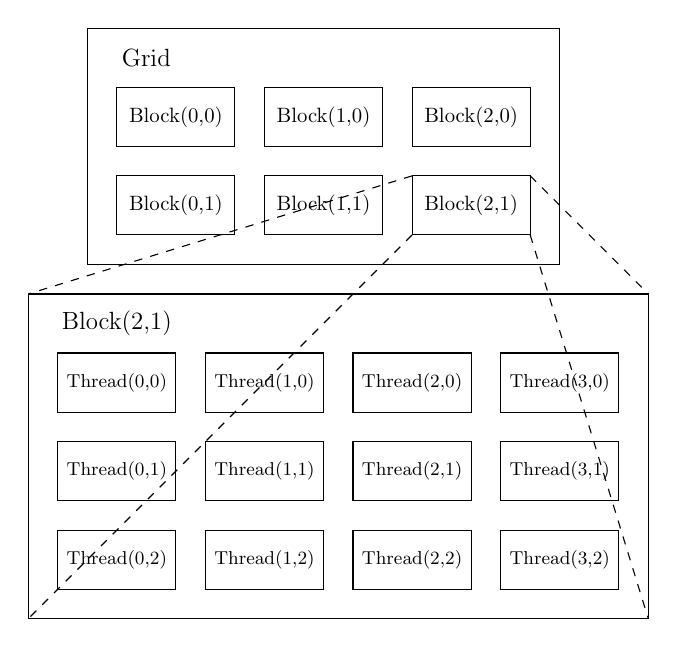
\begin{tikzpicture}[scale=0.75, transform shape]
\def\TextBox#1#2#3{
\draw  (#1,#2) rectangle (#1+2,#2+1);
\node at (#1+1, #2+0.5) {#3};
}

\foreach \x in {0,...,2}
  \foreach \y in {0,...,1}
  {
    \TextBox{\x*2.5+1}{-\y*1.5+3}{Block(\x,\y)}
  }
\draw  (0.5,5) rectangle (8.5,1);
\node at (1.5,4.5) {\large Grid};

\foreach \x in {0,...,3}
  \foreach \y in {0,...,2}
  {
    \TextBox{\x*2.5}{-\y*1.5-1.5}{\small Thread(\x,\y)}
  }
\draw  (-0.5,0.5)  rectangle (10,-5);
\node at (1,0) {\large Block(2,1)};

\draw [dashed]  (6,2.5) edge (-0.5,0.5);
\draw [dashed]  (8,2.5) edge (10,0.5);
\draw [dashed]  (6,1.5) edge (-0.5,-5);
\draw [dashed]  (8,1.5) edge (10,-5);
\end{tikzpicture}
\caption[线程组层次结构示意图]{\label{fig:gpu.cuda.blocks}线程组层次结构示意图
\cite{cudadoc-cprogrammingguide}}
\end{figure}

同一个global函数调用时所涉及的线程均使用global函数的参数作为输入,
CUDA提供threadIdx、blockIdx等变量在代码中区分各个线程。
线程以Block为单元分配给GPU上的各个SMX独立执行,
Block之间没有任何直接的同步方式,
程序员不需要知道也不应该猜测各Block是如何在各个SMX执行的。
需要说明的是:强行使用显存作为Block间的同步可能会导致各SMX死锁。
实际Block间同步的最主要方式就是等待该global函数执行完,
此时所有Block状态都是确定的,即已经执行完。

这样GPU或驱动就可以根据实际GPU核心上的SMX数量来具体配置各Block是如何在SMX上执行的,
使得当SM数量不超过Block数量时global函数有了一定的并行扩展性,
见\floatref{fig:gpu.cuda.scalability}。
由于每个Block是运行在一个实际SMX上的,
所以SMX的寄存器、共享存储空间等资源会对Block的大小(包含的Thread数量)有一定的限制,
而CUDA对Grid大小(包含的Block数量)的限制则很小。
NVIDIA这样做是为了通过强制程序员对计算任务进行分割的方式获得了一定的程序并行扩展性,
同时也简化了同一系列不同规格GPU的设计,即通过增减SMX的数量来控制GPU计算能力。

\begin{figure}
\centering
\begin{tikzpicture}[scale=0.6, transform shape]
\def\TextBox#1#2#3{
\draw  (#1,#2) rectangle (#1+2,#2+1);
\node at (#1+1, #2+0.5) {#3};
}

\foreach \x in {0,...,3}
  \foreach \y in {0,...,1}
  {
    \TextBox{\x*2.5+1}{-\y*1.5+3}{Block(\x,\y)}
  }
\draw  (0.5,5) rectangle (11,1);
\node at (3,4.5) {\large Kernel函数的Grid};

\draw [dashed] (-3,-4) -- (16.5,-4);

\draw  (-1,-3.5) rectangle (4.5,-1);
\node at (1.5,-1.5) {\large 2个SMX的GPU};
\draw [-latex new, arrow head=3mm] (7,1) -- (9.5,-1);
\foreach \x in {0,...,1}
{
  \TextBox{\x*2.5-0.5}{-3}{SMX \x}
}
\foreach \t in {0,...,3}
{
  \foreach \x in {0,...,1}
  {
    \TextBox{\x*2.5-0.5}{-\t*2-6}{Block(\t,\x)}
  }
  \draw  (-1,-\t*2-4.75) rectangle (4.5,-\t*2-6.25);
}

\draw  (5.5,-3.5) rectangle (16,-1);
\node at (8,-1.5) {\large 4个SMX的GPU};
\draw [-latex new, arrow head=3mm] (3.5,1) -- (2,-1);
\foreach \x in {0,...,3}
{
  \TextBox{\x*2.5+6}{-3}{SMX \x}
}
\foreach \t in {0,...,1}
{
  \foreach \x in {0,...,3}
  {
    \TextBox{\x*2.5+6}{-\t*2-6}{Block(\x,\t)}
  }
  \draw  (5.5,-\t*2-4.75) rectangle (16,-\t*2-6.25);
}

\draw [dashed,-latex new, arrow head=3mm] (-1.5,-4.5) -- (-1.5,-13);
\foreach \t in {0,...,3}
{
  \node at  (-2.5,-\t*2-5.5) {\Large t=\t};
}

\draw (5,-0.5) -- (5,-12.5);
\end{tikzpicture}
\caption[CUDA程序的扩展性示意图]{\label{fig:gpu.cuda.scalability}CUDA程序的扩展性示意图
\cite{cudadoc-cprogrammingguide}}
\end{figure}

总的来说,GPU核心相当于一组不能单独编程的、以显存作为共享存储器的、带有自动负载平衡的小型向量机组。


\subsection{CUDA的GPU设备模型}

\begin{figure}
\centering
\begin{tikzpicture}[scale=0.75, transform shape]
%15*SMX
\def\SMX#1#2{
\draw  (#1+0, #2) rectangle (#1+1, #2+1);
\node at (#1+0.5, #2+0.5) {\small SMX};
}
\def\len{1.5}
\foreach \x in {0,...,8}
{ \SMX{\x*\len}{0} }
\foreach \x in {0,...,7}
{ \SMX{\x*\len+0.75}{-3} }

%L2 Cache
\draw  (0,-0.5) rectangle (13,-1.5);
\node at (6.5,-1) {L2缓存};


\def\Memory#1#2{
\draw  (#1,#2) rectangle (#1+2,#2+1);
\node at (#1+1,#2+0.5) {\small 显存控制器};
}
\foreach \i in {0,1,2}
{ \Memory{-2.5}{-\i*1.5} }
\foreach \i in {0,1,2}
{ \Memory{13.5}{-\i*1.5} }

\draw  (-2.5,2) rectangle (15.5,1.5);
\node at (6.5,1.75) {线程调度器(GigaThread Engine)};

\draw  (-2.5,3) rectangle (15.5,2.5);
\node at (6.5,2.75) {PCI Express 3.0接口};

\draw  (-3,4) rectangle (16,-3.5);
\node at (-1.5,3.5) {\Large GK110};
\end{tikzpicture}
\caption[GK110结构示意图]{\label{fig:gpu.cuda.gk110}GK110结构示意图
\cite{cudadoc-KeplerGK110ArchitectureWhitepaper}}
\end{figure}

GPU是由多个SMX组成的,例如Kepler架构GK110核心
(见\floatref{fig:gpu.cuda.gk110})就包含15个SMX,
其中每个SMX(见\floatref{fig:gpu.cuda.smx})
含有192个CUDA Core单元(支持单精度、整数计算,图示中Core)、
64个双精度浮点计算单元(图示中DP Unit)、
32个特殊函数计算单元(图示中SFU)、
32个读取/存储单元(图示中LD/ST),
4个Wrap调度器,65536个32bit寄存器。
SMX以32个Thread为一组(称为wrap)来调度Block中的线程,
每个SMX有4个wrap调度器和8个指令分派单元,这使得SMX可以同时执行4个wrap,
每个周期中每个wrap最多可以有两条不相关的指令被同时分派。
\cite{cudadoc-KeplerGK110ArchitectureWhitepaper}

\begin{figure}
\centering
%\includegraphics[scale=0.6]{smx.png}
\begin{tikzpicture}[scale=0.7, transform shape]
\def\TextBox#1#2#3#4
{
  \draw (#1,#2) rectangle (#1+#3,#2+1);
  \node at (#1+#3/2, #2+0.5) {#4};
}

\def\CoreLine#1#2
{
\foreach \i in {0,...,2}
{ \TextBox{#1+\i*1.5+0}{#2+0}{1}{Core} }
\TextBox{#1+4.5}{#2+0}{2}{DP Unit}

\foreach \i in {0,...,2}
{ \TextBox{#1+\i*1.5+7}{#2+0}{1}{Core} }
\TextBox{#1+11.5}{#2+0}{2}{DP Unit}

\TextBox{#1+14}{#2+0}{1.5}{LD/ST}
\TextBox{#1+16}{#2+0}{1}{SFU}
}

\CoreLine{0}{0}

\CoreLine{0}{-4}

\draw [decorate, decoration={brace, amplitude=10pt}] (-0.5,-4.25) -- (-0.5,1.25);
\node [left]at (-1,-1.5) {\large 32组};
\draw [loosely dashed] (0.5,-0.5) -- (0.5,-2.5);
\draw [loosely dashed] (8,-0.5) -- (8,-2.5);
\draw [loosely dashed] (16.5,-0.5) -- (16.5,-2.5);

\draw  (-0.5,2.5) rectangle (17.5,1.5);
\node at (8,2) {\large 寄存器文件(65536个 32bit寄存器)};

\foreach \x in {0,...,3}
{
  \def\xlen{4.5}
  \draw  (\x*\xlen-0.25,4) rectangle (\x*\xlen-0.25+4,3);
  \node  at (\x*\xlen+1.75,3.5) {\large Wrap调度器}; 
}
\draw  (-0.5,4.5) rectangle (17.5,5.5);
\node at (8,5) {\large 指令缓存};

\draw  (17.5,-4.5) rectangle (-0.5,-5.5);
\draw  (17.5,-6) rectangle (-0.5,-7);
\draw  (17.5,-7.5) rectangle (-0.5,-8.5);
\node at (8,-5) {\large 内部互联网络};
\node at (8,-6.5) {\large 64KB 共享存储区 / L1 缓存};
\node at (8,-8) {\large 48KB 只读数据缓存};

\foreach \x in {0,...,7}
{
  \foreach \y in {0,1}
  {
    \draw  (\x*2.25-0.5,-\y*1.5-9) rectangle (\x*2.25+1.5,-\y*1.5-10);
    \node at (\x*2.25+0.5,-\y*1.5-9.5) {纹理单元};
  }
}

\draw  (-3,-12) rectangle (18,6.5);
\node [right] at (-2.5,6) {\Large SMX};
\end{tikzpicture}
\caption[SMX结构示意图]{\label{fig:gpu.cuda.smx}SMX结构示意图
\cite{cudadoc-KeplerGK110ArchitectureWhitepaper}}
\end{figure}

SMX的存储器结构较为复杂,通用存储器的结构见\floatref{fig:gpu.cuda.memory},
其中寄存器部分和传统程序一样,并不直接对程序员可见,由CUDA编译器进行分配,
L1缓存、L2缓存对程序员也不是直接可见的,会在访问显存时自动进行调度。

\begin{figure}
\centering
\begin{tikzpicture}[scale=0.8, transform shape]

\draw  (0,3) ellipse (1 and 0.5);
\node at (0,3) {Thread};

\draw  (-1.5,0.5) rectangle (1.5,1.5);
\node at (0,1) {L1缓存};

\draw  (-5,0.5) rectangle (-2,1.5);
\node at (-3.5,1) {共享存储区};

\draw  (2,0.5) rectangle (5,1.5);
\node at (3.5,1) {只读数据缓存};

\draw [latex new-latex new, arrow head=3mm] (0,2.5) -- (0,1.5);
\draw [latex new-latex new, arrow head=3mm] (-0.5,2.5) -- (-3.5,1.5);
\draw [latex new-, arrow head=3mm] (0.5,2.5) -- (3.5,1.5);

\draw  (-5,-1.5) rectangle (5,-0.5);
\node at (0,-1) {\large L2缓存};
\draw [latex new-latex new, arrow head=3mm](0,0.5) -- (0,-0.5);
\draw [latex new-, arrow head=3mm](3.5,0.5) -- (3.5,-0.5);

\draw  (-5,-3.5) rectangle (5,-2.5);
\node at (0,-3) {\large 显存};
\draw [latex new-latex new, arrow head=3mm](0,-1.5) -- (0,-2.5);

\draw [decorate, decoration={brace, amplitude=7pt}] (-5.5,0) -- (-5.5,4);
\node [left] at (-5.75,2) {\large SMX};

\draw [decorate, decoration={brace, amplitude=7pt}] (-7,-2) -- (-7,4);
\node [left] at (-7.5,1) {\large GK110};

\draw (-5,2.5) rectangle (-2,3.5);
\node at (-3.5,3) {寄存器};
\draw [latex new-latex new, arrow head=3mm] (-1,3) -- (-2,3);
\end{tikzpicture}
\caption[Kepler存储器结构示意图]{\label{fig:gpu.cuda.memory}Kepler存储器结构示意图
\cite{cudadoc-KeplerGK110ArchitectureWhitepaper}}
\end{figure}

Global函数和device函数可以通过指针直接访问共享存储区、显存。
共享存储区位于SMX内,和L1缓存共用64KB空间,
在global函数启动时可以对共享存储区/L1缓存的分配进行设置,
分配的方式有:16KB/48KB、32KB/32KB(限Kepler架构)、48KB/16KB三种。
\cite{cudadoc-KeplerGK110ArchitectureWhitepaper}

在SMX上运行的Block中的所有线程共享SMX全部的65536个32位寄存器,
一旦分配完成,每个Thread线程就只能使用自己所有的寄存器,其他的寄存器则不可见。
每个Thread需要使用的寄存器数量由CUDA编译器控制。

共享存储区则对同一个Block内所有的线程可见,是同一个Block内的Thread协作、通讯的主要方式,
每个Block使用的共享存储区的大小在global函数启动时进行配置。

只读数据缓存可以用来加速在global函数运行过程中保持不便的数据的读取,
程序员可以通过带有const  \_\_restrict\_\_标识的指针进行访问,
也可以通过纹理模式访问。在Fermi及之前的架构中,该部分缓存只能通过纹理方式使用。
\cite{cudadoc-KeplerGK110ArchitectureWhitepaper}



\section{其他GPU编程技术简介}

\subsection{OpenCL}

在以CUDA为代表的各种硬件相关的GPU、众核编程技术发展之后,
非营利性组织Khronos提出异构平台计算的开放标准OpenCL。

在GPU通用计算领域起步较晚的AMD公司(原ATI公司被AMD收购)
放弃设计一个CUDA这样专为自己生产的GPU编程的编程技术,
直接采用OpenCL作为其GPU的主要开发技术。

OpenCL在很多设备概念、编程模型上照搬较为成熟的CUDA的设计,
但和CUDA相比仍有较大差异。

CUDA程序的编译过程主要发生在主程序开发过程中,CUDA C/C++编译器首先处理CUDA程序的源代码,
把代码分为GPU端和CPU端两部分,CPU端的代码交给GCC/MSVC等传统编译器进行编译,
GPU端的代码则由自己处理,生成相应的GPU PTX代码、主机端调用代码等部分,
最后和程序的其他部分链接成一个主程序。
这其中的PTX代码类似“GPU上的汇编代码”,实际上更接近于Java编译后的字节码,
PTX代码在运行时由主机端驱动程序编译成实际GPU的硬件指令交给GPU运行。
通过增加PTX这一层抽象,NVIDIA使得程序能够在GPU ISA(Instruction Set Architecture)
设计发生变化时仍然可以直接运行。

OpenCL代码语法和CUDA一样以C为蓝本,但并不和普通的C代码混在一起,
而是直接以文本形式保存于程序或其他数据文件中,
在运行时由硬件驱动进行编译生成实际硬件代码运行。
所以说OpenCL程序的编译过程主要发生在运行时。

现在支持OpenCL的主要硬件/厂商有:\cite{opencl-conformant-products}
\begin{enumerate}[1)]
\item Intel x86 CPU(及内嵌的Intel HD Graphics集成显卡)
\item AMD CPU/APU
\item AMD显卡
\item NVIDIA显卡
\item Intel MIC(Many Integrated Core) Architecture
\item ARM
\end{enumerate}
相对来说,AMD显卡和MIC上的OpenCL支持较好,因为这是它们上的主要编程方式,
NVIDIA对OpenCL的支持略差,某些情况下可能会有性能明显下降的情况。


\subsection{C++ AMP}

C++ AMP全称C++ Accelerated Massive Parallelism
\cite{cppamp}
\subsection{OpenACC与OpenMP}
